% Requires amsmath and graphicx in the manuscript preamble.
% Keep the three accompanying figure files on the manuscript graphics path.
% Citation keys from the supplied manuscript are preserved.

\subsection{Experimental Setup}
The experiment was performed at the HED--HiBEF instrument at the European XFEL to investigate small-angle X-ray scattering (SAXS) asymmetry from copper microwires, with particular emphasis on its dependence on the transverse position of the wire relative to the XFEL beam. X-ray pulses generated by self-amplified spontaneous emission (SASE), with a central photon energy of $8.2\,\mathrm{keV}$, a full width at half maximum (FWHM) pulse duration of approximately $25\,\mathrm{fs}$, a bandwidth of approximately $20\,\mathrm{eV}$, and a total pulse energy of approximately $1.5\,\mathrm{mJ}$, illuminated $10\,\mu\mathrm{m}$-diameter Cu wires perpendicular to the wire axis. The intensity FWHM at the target was approximately $7.11\,\mu\mathrm{m}$.

To investigate the influence of nonuniform illumination on the scattering asymmetry, the wire was scanned transversely across the XFEL beam over an offset range of $-10$ to $+10\,\mu\mathrm{m}$ in steps of $(0.78\pm0.22)\,\mu\mathrm{m}$. The wire offset $x_0$ was defined as the transverse displacement of the wire center relative to the beam axis. Figures~\ref{fig:experimental_setup}(b)--(d) illustrate the beam--wire overlap at offsets of $-5$, $0$, and $+5\,\mu\mathrm{m}$, respectively. Beneath each three-dimensional schematic, the shaded region marks the projected wire cross section, while the Gaussian curve represents the normalized incident intensity centered at $x=0$. At $x_0=-5\,\mu\mathrm{m}$, the beam maximum lies at the right edge of the wire, so that edge receives stronger illumination than the left edge. At $x_0=0$, the beam and wire centers coincide, and the illumination is symmetric about the wire center. At $x_0=+5\,\mu\mathrm{m}$, the beam maximum lies at the left edge, reversing the illumination imbalance. The bottom row shows representative experimental SAXS patterns at offsets of approximately $-4.95$, $0$, and $+4.95\,\mu\mathrm{m}$, respectively, linking the illustrated illumination geometries to the measured scattering distributions. The patterns are displayed in $(q_x,q_y)$ coordinates with a shared logarithmic intensity scale.

SAXS patterns were recorded using a Jungfrau X-ray detector at a target-to-detector propagation distance of $1.31\,\mathrm{m}$. Two highly annealed pyrolytic graphite (HAPG) mirrors, positioned above and below the primary beam path, reflected the SAXS signal onto the detector\cite{Jungfrau} while allowing the transmitted beam to pass through their central gap. Complementary X-ray phase-contrast images were acquired simultaneously at a distance of $6.31\,\mathrm{m}$ using a scintillator screen coupled to an Andor Zyla CMOS camera through a $7.5\times$ microscope objective\cite{Smid2020}. This configuration enabled systematic measurements of the SAXS intensity distribution and its asymmetry as a function of wire offset. Figure~\ref{fig:experimental_setup}(a) shows the experimental arrangement. Detailed experimental conditions are described in our previous publication\cite{Huang2026}.

\begin{figure*}[t]
    \centering
    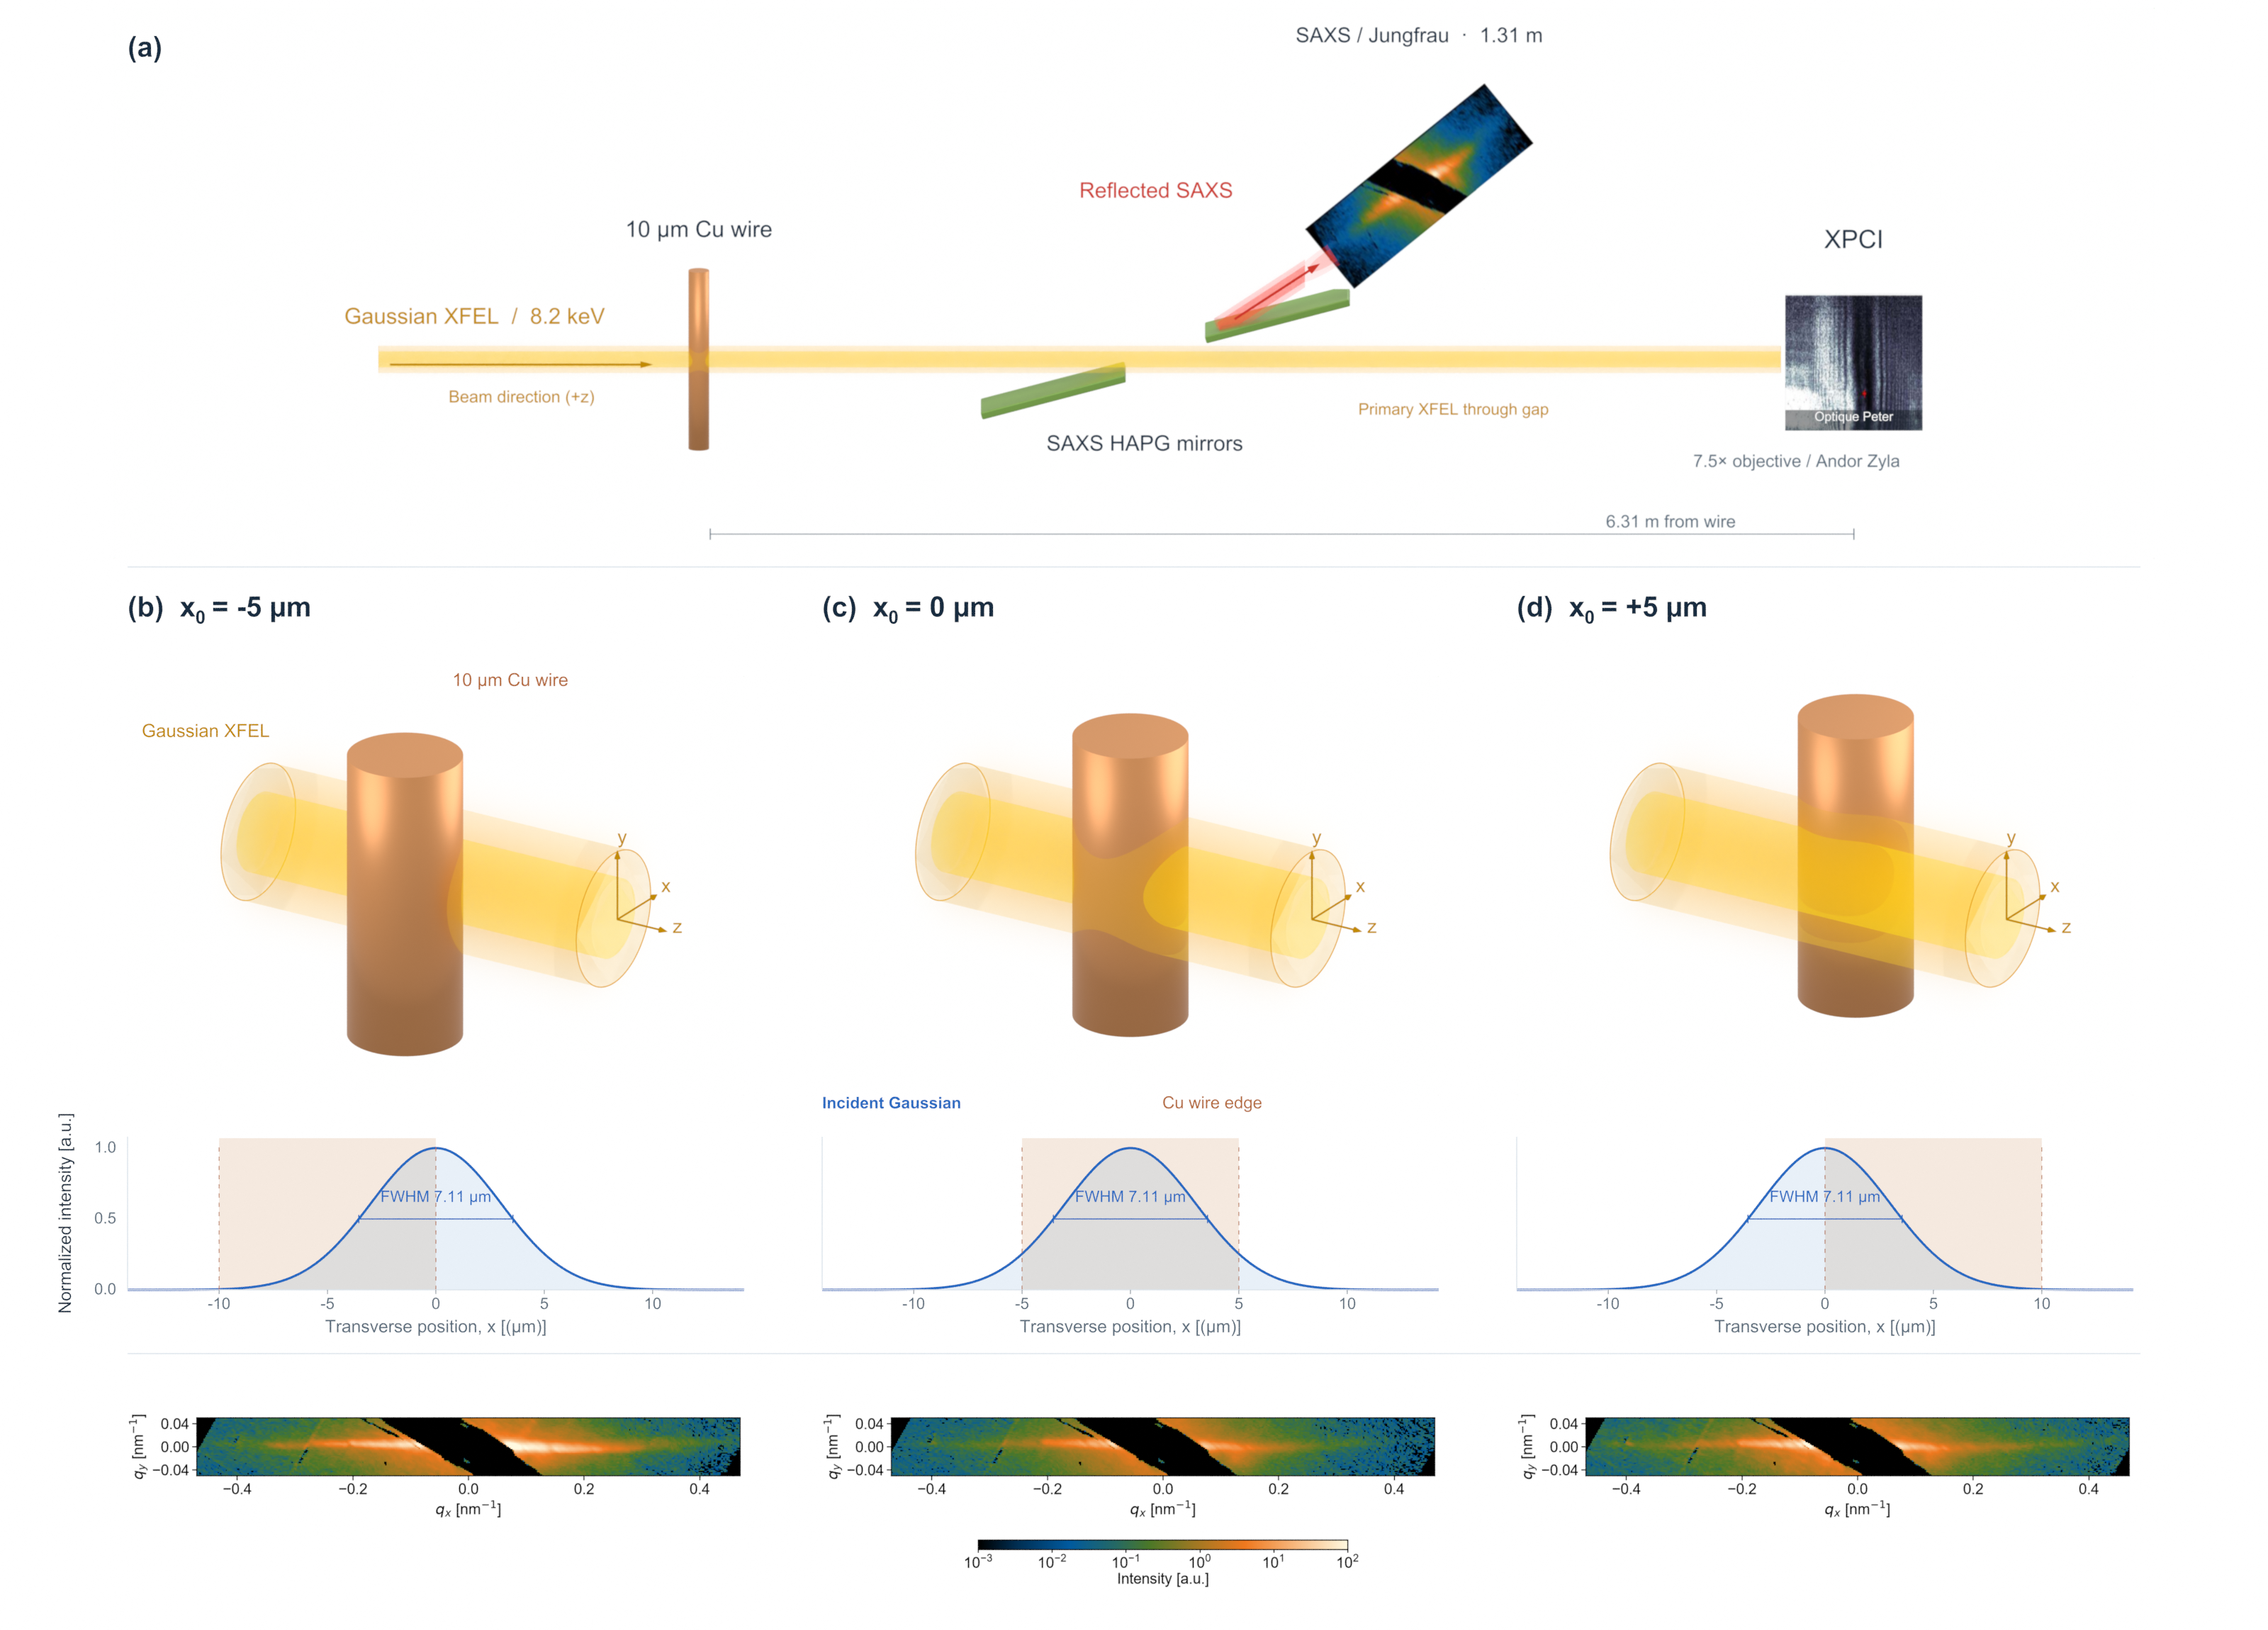
\includegraphics[width=\textwidth]{01_experimental_setup.png}
    \caption{Schematic of the SAXS and XPCI diagnostics, wire-offset geometry, and representative experimental SAXS patterns. (a) An $8.2\,\mathrm{keV}$ XFEL beam illuminates a $10\,\mu\mathrm{m}$-diameter Cu wire. HAPG mirrors direct the SAXS signal to a Jungfrau detector at a propagation distance of $1.31\,\mathrm{m}$, while the primary transmitted beam passes through the gap between the mirrors to the XPCI diagnostic, $6.31\,\mathrm{m}$ downstream of the target. The latter uses a scintillator screen and a $7.5\times$ microscope objective coupled to an Andor Zyla CMOS camera. (b)--(d) Illustrative wire offsets of $-5$, $0$, and $+5\,\mu\mathrm{m}$ relative to the beam axis. The profiles beneath the three-dimensional schematics show the normalized incident Gaussian intensity, with a FWHM of $7.11\,\mu\mathrm{m}$, and the shaded projected wire cross section. The bottom row shows experimental SAXS patterns at the corresponding measured offsets of approximately $-4.95$, $0$, and $+4.95\,\mu\mathrm{m}$, respectively, using a shared logarithmic intensity scale. The three schematic offsets do not coincide with the discrete positions of the simulated scan.}
    \label{fig:experimental_setup}
\end{figure*}

\subsection{SAXS Simulation Configuration and Analysis Workflow}
\label{sec:saxs_simulation}

Small-angle X-ray scattering (SAXS) patterns were simulated using a coherent scalar wave model that accounts for the spatial amplitude and phase of the incident beam, sample transmission, and propagation to the detector. The photon energy was $8.2\,\mathrm{keV}$, corresponding to a wavelength of $\lambda\simeq0.1512\,\mathrm{nm}$. At the sample, the incident beam had a Gaussian intensity profile with a full width at half maximum (FWHM) of $7.11\,\mu\mathrm{m}$. The sample was modeled as a copper cylinder of radius $a=5\,\mu\mathrm{m}$, with its axis parallel to the $y$ axis. The sample plane was located $0.25\,\mathrm{m}$ downstream of the reference beam-waist plane.

\begin{figure*}[t]
    \centering
    
\includegraphics[width=0.96\textwidth]{03_saxs_workflow.pdf}
    \caption{Workflow for the SAXS simulation and asymmetry analysis. (a), (b) The fixed incident field and the translated wire thickness, with independent edge-smoothing widths $\sigma_L=4.67\,\mathrm{nm}$ and $\sigma_R=0\,\mathrm{nm}$, define (c) the sample-exit field. (d) Fresnel propagation retains the sample-plane quadratic phase and yields the detector intensity from a two-dimensional Fourier transform. The additional Fraunhofer approximation is shown for comparison. (e) The ten central detector rows are averaged to obtain a one-dimensional SAXS profile. Left and right intensity sums are evaluated for $q_x<-0.10\,\mathrm{nm}^{-1}$ and $q_x>+0.10\,\mathrm{nm}^{-1}$, respectively, and the left-side fraction $f_L$ is calculated at each wire offset. The colored strip denotes the integration regions and the excluded central interval.}
    \label{fig:saxs_workflow}
\end{figure*}

The simulation and analysis workflow is summarized in Figure~\ref{fig:saxs_workflow}. The fixed incident beam and the asymmetrically smoothed, translated wire are specified in Figures~\ref{fig:saxs_workflow}(a) and \ref{fig:saxs_workflow}(b), respectively. These inputs define the sample-exit field in Figure~\ref{fig:saxs_workflow}(c), which is propagated to obtain the detector intensity in Figure~\ref{fig:saxs_workflow}(d). The resulting SAXS profile is then used to calculate the left-side intensity fraction at each wire offset, as outlined in Figure~\ref{fig:saxs_workflow}(e) and described below. The wire offset $x_0$ was defined as the displacement of the wire center along $x$, perpendicular to the wire axis, relative to the beam center at $x=0$. Positive offsets corresponded to translation in the positive $x$ direction. The incident beam and the detector coordinate system remained fixed throughout the scan. The simulated wire positions were
\begin{equation}
x_0^{(n)}=x_{\min}+n\Delta x_0,
\qquad n=0,\ldots,42,
\end{equation}
where $x_{\min}=-10.0\,\mu\mathrm{m}$ and $\Delta x_0=0.48\,\mu\mathrm{m}$, giving 43 positions from $-10.0$ to $+10.16\,\mu\mathrm{m}$.

For a wire centered at $x=0$, the ideal thickness projected along the beam direction was
\begin{equation}
t_0(x)=
\begin{cases}
2\sqrt{a^2-x^2}, & |x|\leq a,\\
0, & |x|>a.
\end{cases}
\label{eq:saxs_ideal_thickness}
\end{equation}
Before calculating the SAXS, the projected thickness was smoothed along $x$ using independent Gaussian widths for the two wire edges. For a width $\sigma>0$, the smoothed reference profile was
\begin{equation}
\begin{aligned}
t_\sigma(x)
&=\int_{-\infty}^{\infty}G_\sigma(x-u)\,t_0(u)\,\mathrm{d}u,\\
G_\sigma(\xi)
&=\frac{1}{\sqrt{2\pi}\sigma}
\exp\!\left(-\frac{\xi^2}{2\sigma^2}\right),
\end{aligned}
\label{eq:saxs_gaussian_smoothing}
\end{equation}
where $\sigma$ is the standard deviation of the Gaussian kernel and $\xi$ is the spatial separation between two points. The case $\sigma=0$ denotes the ideal profile $t_0(x)$ without additional Gaussian smoothing. The convolution averages neighboring thickness values and broadens the steep transition at each wire boundary.

To allow different smoothing at the left and right edges, two independently convolved profiles were joined at the wire center:
\begin{equation}
t_{\sigma_L,\sigma_R}(x)=
\begin{cases}
t_{\sigma_L}(x), & x\leq0,\\
t_{\sigma_R}(x), & x>0.
\end{cases}
\label{eq:saxs_asymmetric_smoothing}
\end{equation}
The subscripts $L$ and $R$ refer to the negative- and positive-$x$ sides of the centered wire, respectively. The final simulation configuration used $\sigma_L=4.67\,\mathrm{nm}$ and $\sigma_R=0\,\mathrm{nm}$ at every scan position. Thus, the left edge was Gaussian-smoothed, while the right edge retained the ideal projected profile within the discretized model.

Figure~\ref{fig:wire_edge_smoothing} compares the projected thickness near $x=\pm5\,\mu\mathrm{m}$ for $(\sigma_L,\sigma_R)=(0,0)$, $(3,3)$, $(4,4)$, $(4.67,0)$, $(6,8)$, and $(8,14)\,\mathrm{nm}$. The first three pairs provide symmetric reference profiles, whereas the remaining pairs illustrate independent broadening of the two edges. For the final pair $(4.67,0)\,\mathrm{nm}$, only the left boundary is broadened; the right boundary coincides with the unsmoothed reference. These fixed, unequal edge widths introduce a structural asymmetry in addition to the illumination imbalance produced by translating the wire across the Gaussian beam.

\begin{figure*}[t]
    \centering
    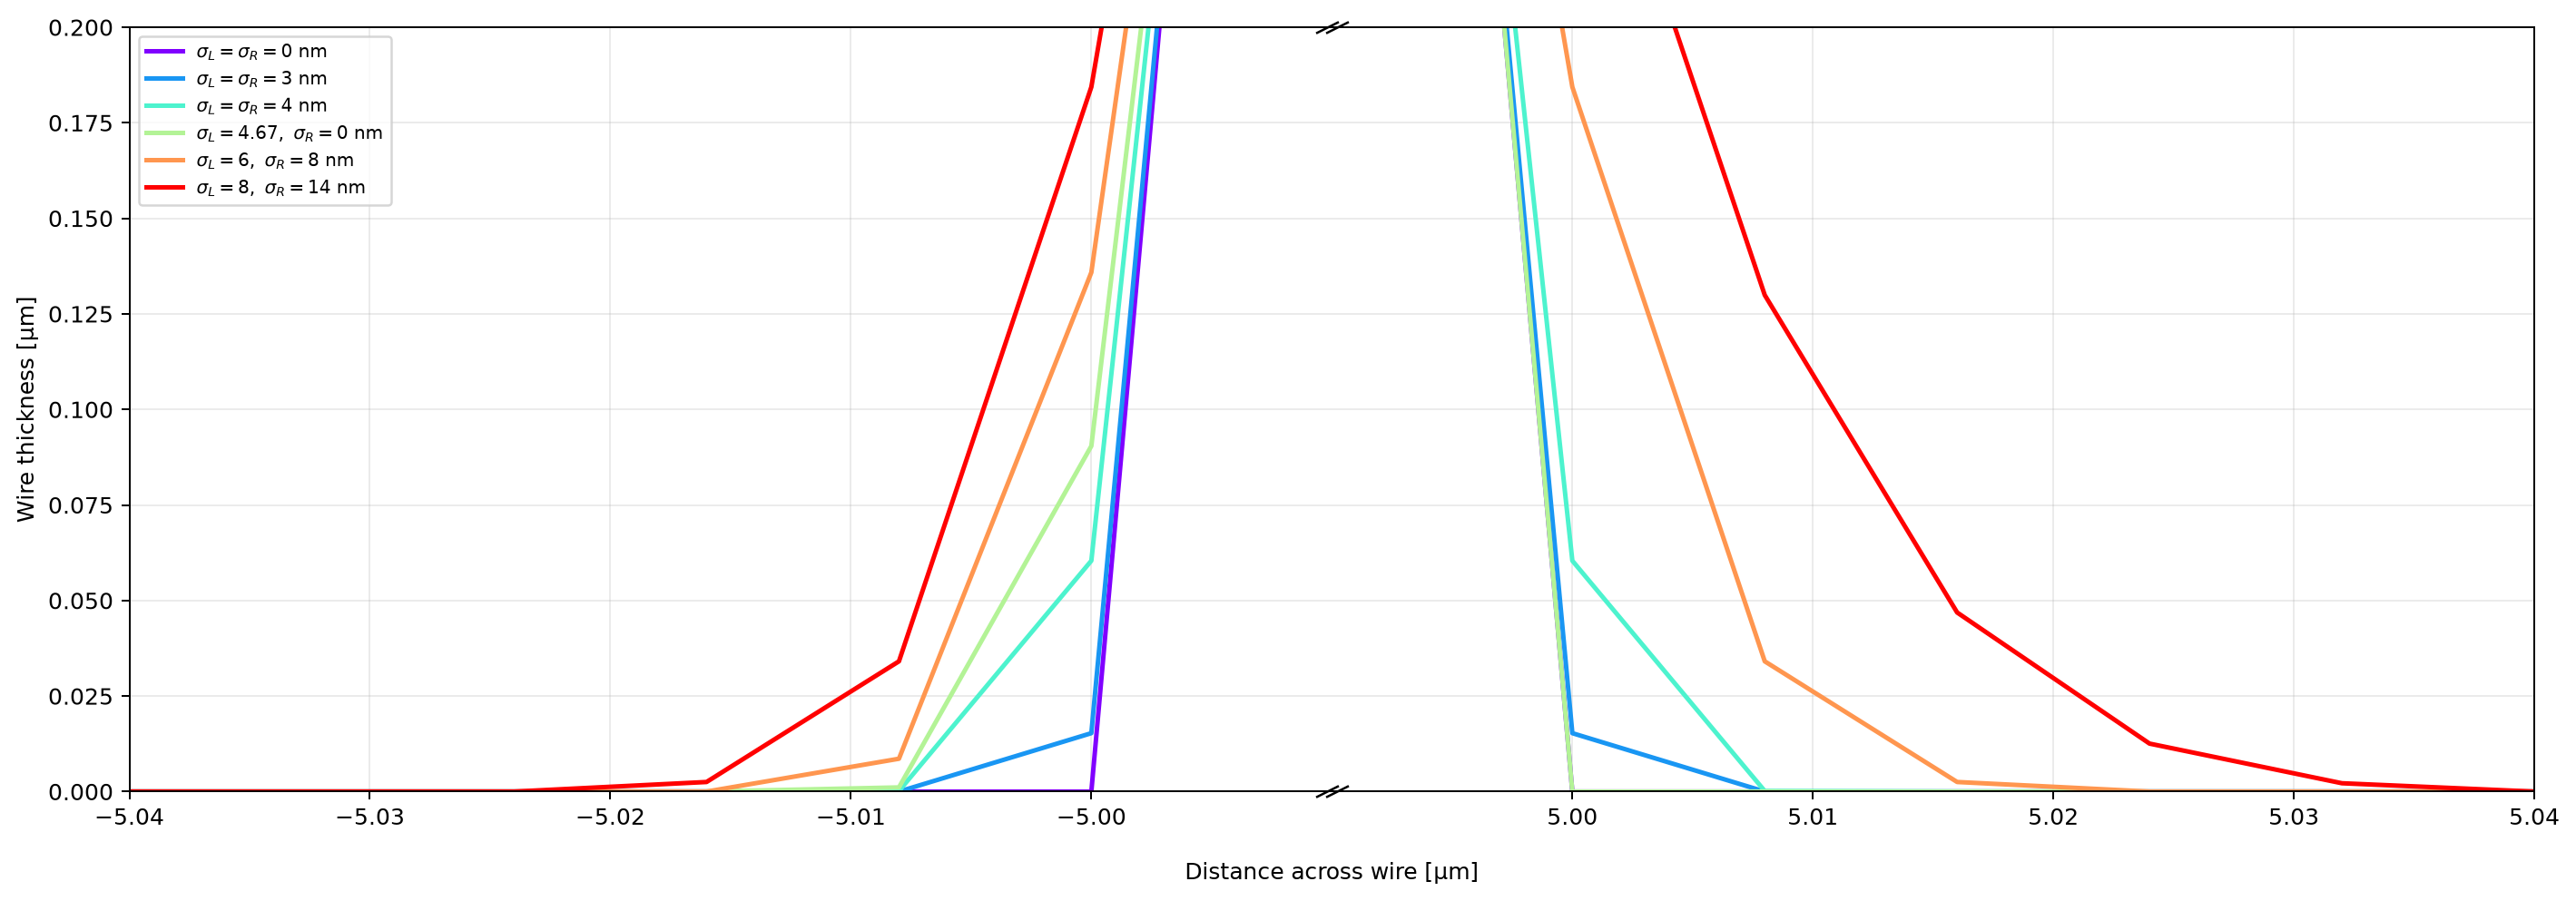
\includegraphics[width=\textwidth,height=0.68\textheight,keepaspectratio]{02_asymmetric_sigma_wire_edges.png}
    \caption{Projected thickness profiles near the left and right edges of a centered $10\,\mu\mathrm{m}$-diameter Cu wire for Gaussian smoothing-width pairs $(\sigma_L,\sigma_R)=(0,0)$, $(3,3)$, $(4,4)$, $(4.67,0)$, $(6,8)$, and $(8,14)\,\mathrm{nm}$. A zero width denotes the ideal projected profile without additional Gaussian smoothing. The final simulation configuration uses $\sigma_L=4.67\,\mathrm{nm}$ and $\sigma_R=0\,\mathrm{nm}$, producing a broadened left edge and an unsmoothed right edge. The horizontal-axis break omits the central part of the wire.}
    \label{fig:wire_edge_smoothing}
    \label{fig:symmetric_sigma}
\end{figure*}

At each scan position, the centered profile with independently smoothed edges was translated along $x$ and taken to be uniform along the wire axis:
\begin{equation}
t_n(x,y)=t_{\sigma_L,\sigma_R}\!\left(x-x_0^{(n)}\right).
\label{eq:saxs_translated_thickness}
\end{equation}
The corresponding displacement in target-grid pixels was
\begin{equation}
s_n=\frac{x_0^{(n)}}{\Delta x_{\mathrm{target}}},
\qquad \Delta x_{\mathrm{target}}=8\,\mathrm{nm},
\label{eq:displacement}
\end{equation}
so each scan increment of $0.48\,\mu\mathrm{m}$ corresponded to 60 target-grid pixels.

As shown in the field-construction stage of Figure~\ref{fig:saxs_workflow}(c), the translated thickness profile determined the sample attenuation and phase shift. These quantities were interpolated onto the beam grid and combined with the fixed incident field. The complex field immediately downstream of the sample was
\begin{equation}
\begin{aligned}
E_{\mathrm{exit}}^{(n)}(x,y)
&=E_{\mathrm{in}}(x,y)
\exp\!\left[-\frac{\mu t_n(x,y)}{2}\right]\\
&\quad\times\exp\!\left[-ik\delta t_n(x,y)\right],
\end{aligned}
\label{eq:saxs_exit_field}
\end{equation}
where $k=2\pi/\lambda$, $\mu$ is the linear intensity attenuation coefficient, and $\delta$ is the refractive index decrement. The latter two quantities were supplied by the copper material model at the specified photon energy. 

Propagation from the sample to the detector can be expressed by the Rayleigh--Sommerfeld diffraction integral. For a sample-to-detector distance $Z$, the detector field is
\begin{equation}
\begin{aligned}
E_D^{(n)}(X,Y)
&=\frac{1}{i\lambda}
\iint E_{\mathrm{exit}}^{(n)}(x,y)\frac{Z}{R^2}\\
&\quad\times\left(1+\frac{i}{kR}\right)e^{ikR}\,\mathrm{d}x\,\mathrm{d}y,
\end{aligned}
\label{eq:saxs_rayleigh_sommerfeld}
\end{equation}
where $(x,y)$ and $(X,Y)$ are transverse coordinates in the sample and detector planes, respectively, and
\[
R=\sqrt{Z^2+(X-x)^2+(Y-y)^2}.
\]
The calculation used the paraxial Fresnel approximation to this integral. Since $kR\gg1$, the term $i/(kR)$ was neglected. Under the small-angle assumption, the amplitude factor was approximated by $Z/R^2\simeq1/Z$, and the propagation distance in the phase was retained to quadratic order:
\[
R\simeq Z+\frac{(X-x)^2+(Y-y)^2}{2Z}.
\]
The resulting detector field is
\begin{multline}
E_D^{(n)}(X,Y)
=\frac{e^{ikZ}}{i\lambda Z}
\iint E_{\mathrm{exit}}^{(n)}(x,y)\\
{}\times\exp\!\left[\frac{ik}{2Z}\bigl((X-x)^2+(Y-y)^2\bigr)\right]
\,\mathrm{d}x\,\mathrm{d}y.
\label{eq:saxs_fresnel_real_space}
\end{multline}

Expanding the squares separates the propagation kernel into quadratic phase factors in the sample and detector coordinates and a cross term, $\exp[-ik(Xx+Yy)/Z]$. The cross term has the Fourier-transform form $\exp[-i(q_x x+q_y y)]$, with
\begin{equation}
q_x=\frac{kX}{Z},
\qquad
q_y=\frac{kY}{Z}.
\label{eq:saxs_detector_q_mapping}
\end{equation}
Thus, the Fresnel integral can be evaluated using a single two-dimensional Fourier transform. Defining the phase-modified sample field $U_n(x,y)$ gives
\begin{equation}
\begin{aligned}
U_n(x,y)
&=E_{\mathrm{exit}}^{(n)}(x,y)
\exp\!\left[\frac{ik(x^2+y^2)}{2Z}\right],\\
\widetilde{U}_n(q_x,q_y)
&=\mathcal{F}_{x,y}\{U_n\}(q_x,q_y),\\
E_D^{(n)}(X,Y)
&=\frac{e^{ikZ}}{i\lambda Z}
\exp\!\left[\frac{ik(X^2+Y^2)}{2Z}\right]\\
&\quad\times\widetilde{U}_n\!\left(\frac{kX}{Z},\frac{kY}{Z}\right).
\end{aligned}
\label{eq:saxs_fresnel_field}
\end{equation}
The transform $\mathcal{F}_{x,y}$ uses the kernel $\exp[-i(q_x x+q_y y)]$. The coordinates $(q_x,q_y)$ are angular spatial frequencies, and Equation~\eqref{eq:saxs_detector_q_mapping} maps them to physical detector coordinates $(X,Y)$.

The detector intensity was calculated from the squared magnitude of the propagated field. The global phase and detector-plane quadratic phase factors do not affect the intensity. Apart from an overall normalization,
\begin{equation}
I_D^{(n)}(X,Y)
\propto
\left|
\widetilde{U}_n\!\left(\frac{kX}{Z},\frac{kY}{Z}\right)
\right|^2.
\label{eq:saxs_fresnel}
\end{equation}
The sample-plane quadratic phase is included in $U_n$ and retained in the Fourier transform. For comparison, Fraunhofer propagation makes an additional far-field approximation to the Fresnel integral. If the sample-plane quadratic phase varies negligibly over the significant illuminated field, then
\begin{equation}
\begin{aligned}
\exp\!\left[\frac{ik(x^2+y^2)}{2Z}\right]&\simeq1,\\
U_n(x,y)&\simeq E_{\mathrm{exit}}^{(n)}(x,y).
\end{aligned}
\label{eq:saxs_fraunhofer_condition}
\end{equation}
For a characteristic illuminated transverse radius $\ell$, this requires $\pi\ell^2/(\lambda Z)\ll1$. Under this additional far-field (Fraunhofer) approximation, the intensity becomes
\begin{equation}
I_{D}^{(n)}(X,Y)\propto
\left|
\mathcal{F}_{x,y}\!\left\{E_{\mathrm{exit}}^{(n)}\right\}
\!\left(\frac{kX}{Z},\frac{kY}{Z}\right)
\right|^2.
\label{eq:saxs_fraunhofer}
\end{equation}

The simulations retained the sample-plane quadratic phase and used the Fresnel expression in Equation~\eqref{eq:saxs_fresnel}. The propagation distance was $Z=1.31\,\mathrm{m}$. The calculation used a $4096\times4096$ grid with sample-plane spacings of $\Delta x=\Delta y=8\,\mathrm{nm}$. With $N=4096$ points along each axis, the corresponding numerical detector spacing was $\Delta X=\Delta Y=\lambda Z/(N\Delta x)\simeq6.04\,\mu\mathrm{m}$. For the subsequent SAXS analysis, the horizontal detector position was expressed as the signed coordinate $q_x=kX/Z$, measured relative to the optical axis.

Following the analysis step in Figure~\ref{fig:saxs_workflow}(e), the detector intensity was reduced to a one-dimensional SAXS profile, $\overline{I}_n(q_x)$, by averaging the ten central detector rows. To prevent the much stronger central intensity from dominating the analysis, the region $|q_x|\leq q_{\min}$ was excluded, where $q_{\min}=0.10\,\mathrm{nm}^{-1}$. The integration regions were defined relative to the fixed optical axis at $q_x=0$ and were identical at every wire offset. The colored strip in Figure~\ref{fig:saxs_workflow}(e) identifies the left and right regions used to form the intensity sums
\begin{equation}
\begin{aligned}
S_L^{(n)}&=\sum_{q_x<-q_{\min}}\overline{I}_n(q_x),\\
S_R^{(n)}&=\sum_{q_x>+q_{\min}}\overline{I}_n(q_x).
\end{aligned}
\label{eq:saxs_side_sums}
\end{equation}
The left and right sums therefore include $q_x<-0.10\,\mathrm{nm}^{-1}$ and $q_x>+0.10\,\mathrm{nm}^{-1}$, respectively.

At each wire offset, the left-side intensity fraction was calculated as
\begin{equation}
f_L^{(n)}=
\frac{S_L^{(n)}}{S_L^{(n)}+S_R^{(n)}}.
\label{eq:saxs_left_fraction}
\end{equation}
Thus, $f_L=0.5$ indicates equal intensity sums in the selected regions, whereas values above or below $0.5$ indicate a larger left or right contribution, respectively. Because the final wire model has unequal edge-smoothing widths, symmetric illumination at zero wire offset does not by itself require $f_L=0.5$.
